\documentclass[a4paper, twoside]{report}
%% Language and font encodings
\usepackage[english]{babel}
\usepackage[utf8x]{inputenc}
\usepackage[T1]{fontenc}

%% font size related
% \linespread{1.15}
% \setlength{\parskip}{5pt}

%% Chapter Beautify
\usepackage{titlesec}
% \newcommand{\hsp}{\hspace{20pt}}
% \titleformat{\chapter}[hang]{\Huge\bfseries}{\thechapter\hsp|\hsp}{0pt}{\Huge\bfseries}

%% Very nice Font
\usepackage{palatino}

%% Diagram drawing
\usepackage{tikz}
\usetikzlibrary{shapes.geometric, arrows}

%% Forced float
\usepackage{float}

%% Source code highlight
\usepackage{minted}
\usepackage{listings}

%% figure

%% Code line references
\setminted[haskell]{escapeinside=\#\#, linenos=true, mathescape=true}
\usepackage{caption}
\usepackage{tikz}
\newcommand*\circled[1]{\tikz[baseline=(char.base)]{
            \node[shape=circle,draw,inner sep=1pt, text=white] (char) {#1};}}
\newcommand*\clabel[1]{$\label{#1} \circled{\ref{#1}}$}
\newcommand*\cref[1]{\circled{\ref{#1}}}
\newcommand*\ccaption[2]{
    \caption[.]{
        \centering #1\newline
        \begin{minipage}{\linewidth}
            #2
        \end{minipage}
        \newline
    }
}

\newenvironment{code}{\captionsetup{type=listing}}{}
%% Automatic Reference

% BNF Rule
\usepackage{mathtools,array}
\newenvironment{grammar}[2]
 {\begin{tabular}{@{\qquad}>{$}l<{$}@{\qquad}l@{}}
  \multicolumn{1}{@{}l@{}}{$#1$}&\multicolumn{1}{l@{}}{\hspace{-2em}#2}\\}
 {\end{tabular}}

%% Placeholder picture
\usepackage{mwe}

%% Format Paragraph
\setcounter{secnumdepth}{4}
\titleformat{\paragraph}
{\normalfont\normalsize\bfseries}{\theparagraph}{1em}{}
\titlespacing*{\paragraph}
{0pt}{3.25ex plus 1ex minus .2ex}{1.5ex plus .2ex}

%% Sets page size and margins
\usepackage[a4paper,top=3cm,bottom=2cm,left=3cm,right=3cm,marginparwidth=1.75cm]{geometry}

%% Useful packages
\usepackage{amsmath}
\usepackage{amssymb}
\usepackage{graphicx}
\usepackage{subcaption}
\usepackage[colorinlistoftodos]{todonotes}
\usepackage[colorlinks=true, allcolors=black]{hyperref}

%% Reference for figure, section and source code
\newcommand*{\tabref}[1]{\tablename~\ref{#1}}
\newcommand*{\figref}[1]{\figurename~\ref{#1}}
\newcommand*{\coref}[1]{\lstlistingname~\ref{#1}}
\newcommand*{\secref}[1]{Section~\ref{#1}}

%% Line number
% \usepackage{lineno}
% \linenumbers

%% for example
\usepackage{xspace}
\newcommand*{\eg}{e.g.\@\xspace}

%% Nested list
\usepackage{enumitem}
\setlist[enumerate]{label*=\arabic*.}

%% Haskell 
\newcommand*{\hask}[1]{\mintinline{text}{#1}}

%% https://tex.stackexchange.com/questions/375992/bad-mathchar-with-semantic-package
\usepackage{semantic}

\title{TODO}
\author{Shuhao Zhang}
% Update supervisor and other title stuff in title/title.tex

\begin{document}
\input{title/title.tex}

% TODO
% \begin{abstract}
% TBD
% \end{abstract}

% \renewcommand{\abstractname}{Acknowledgements}
% \begin{abstract}
% TBD
% \end{abstract}

\tableofcontents
% \listoffigures
% \listoftables

\chapter{Introduction} \label{chap:intro}
% define the session typed monad language
% Arrow => seesson typed monadic lagnauge
% Turning data flow into communication 
% compile session-typed monadic language to C
% results => a standalone framework for parallel computation
% high-level arrow code => 1) abstraction layer on top of settiontype language  2) a set of local types to reason so that it's possible reason about the structure of parallel computation 
% as a use case => compile to c
% as a use case => backend for ParAlg
% put the picture in the introduction
% 
% title : session-arrow =>  

\section{Motivation} \label{i:m}
Writing parallel software is not a trivial task. Parallel code is hard to write because it is usually written in low level languages with verbose and non-idiomatic decorations, hard to debug because machines, where code is written, are usually different from machines where code is intended to run and hard to maintain and reuse because even though the underlying algorithms are not changed, multiple version of parallel code is needed to tackle various platform and evolution of architectures.

There are many on-going pieces of research aimed at helping programmers write correct parallel programs smoothly. A common approach is to develop a higher level language and compiles programmes in this language to required parallel code. There are many high-level frameworks for parallel programming (\eg algorithmic skeletons\cite{coleAlgorithmicSkeletonsStructured}, domain-specific languages for parallelism\cite{brownHeterogeneousParallelFramework2011} or famous MapReduce parallel model\cite{liMapReduceParallelProgramming2016}). An example is to use arrow terms (\secref{b:arrows}) to describe data flow implicitly and hence generate parallel code.

The workflow of writing parallel code has evolved from writing it directly in the target platform to writing software in a high-level language designed for parallel computation and then compiling to the target platform. In this project, we present a method to improve the backend of parallel code generation by introducing a monadic domain-specific language to act as a bridge between high-level and target low-level parallel languages.

This specific language needs to be general enough so that it supports multiple high-level parallel programming frameworks. It can be used to generate different parallel code, e.g. MPI \footnote{Message Passing Interface (MPI) is a standardized and portable message-passing standard designed by a group of researchers from academia and industry to function on a wide variety of parallel computing architectures \cite{MessagePassingInterface2018}.}, Cuda. Moreover, it can be interpreted with a simulator to aid debugging parallel programs.

% With the help of this intermediate languages, the implementation complexity is reduced from $O(M \times N)$, where each of the M high-level languages needs to implement N compilers to generate parallel code in N different platforms, to $O(M + N)$, where each compiler of a high-level language implements a translation rule to the intermediate language which implements one compiler and N backend to generate different target languages.

In addition, it couples with multiparty session type (MPST) \cite{coppoGentleIntroductionMultiparty2015}. It takes advantages of properties of MPST to enable aggressive optimisation but ensuring code correctness and allow more meaningful static analysis; \eg cost modelling for parallel programming. % (TODO add more examples of possible kinds of static analysis and reference paper).
\section{Contributions} 
\begin{figure}[ht]
    \centering
    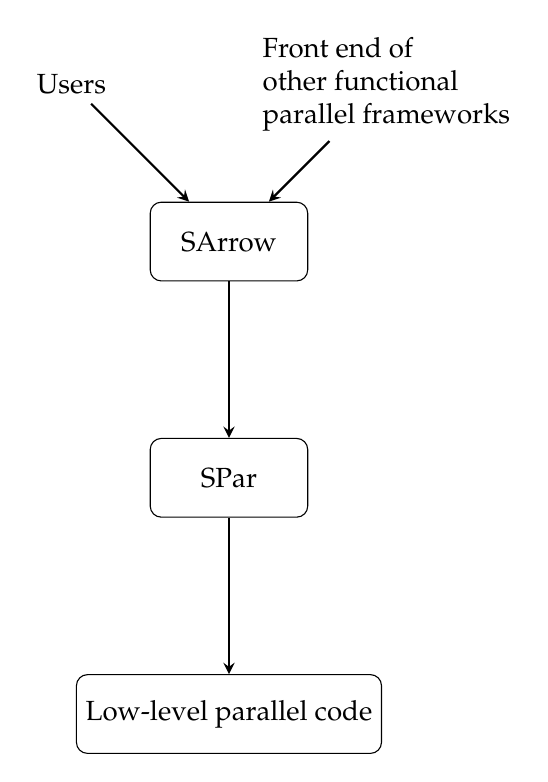
\begin{tikzpicture}[xscale=.5]
    \tikzstyle{proc}  = [rectangle, rounded corners, minimum width=2cm, minimum height=1cm,text centered, draw=black] 
    \tikzstyle{proc1} = [circle,  minimum width=1cm, minimum height=1cm,text centered, draw=black] 
    \tikzstyle{arrow} = [thick,->,>=stealth]
    \node (a) [proc] at (0, 3)  {SArrow};
    \node (b) [proc] at (0, 0)  {SPar};
    \node (c) [proc] at (0, -3) {Low-level parallel code};
    \node (d)  at (-4, 5) {Users};
    \node (e) [align=left] at (4, 5) {Front end of \\ other functional  \\ parallel frameworks};
    \draw[arrow] (a) to (b);
    \draw[arrow] (b) to (c);
    \draw[arrow] (d) to (a);
    \draw[arrow] (e) to (a);
    \end{tikzpicture}
    \caption{Visualization of the workflow}
    \label{intro:fig:workflow}
\end{figure}
The result of project is a embedded high-level framework in Haskell that is capable of generating low-level parallel code. The major contributions are:
\begin{enumerate}
    \item \textbf{Session-typed intermediate language. } We create an intermediate embedded domain specific language (EDSL): SPar: a session typed free monad EDSL for message passing concurrency. This language can be typed by local types, and hence, we can apply multiple results from the multiparty session types to our framework, especially in terms of safety of generated code and reasoning of communication patterns.
    \item \textbf{Intuitive user interface. } One innovation of this project is that we apply the mature Arrow interface for users to express parallel computations. We call the interface SArrow: an arrow interface for writing SPar expressions. It is an abstraction layer on top of SPar, which hides communication primitives from users so that users can express parallel algorithms similar to what they would write for sequential programs.
    \item \textbf{Multiple backends. } We create a backend to generate parallel C code from SPar expressions. The core of the backend is Instr: a low-level EDSL that is independent of target languages. This means that we can support multiple target languages with ease without re-implementing multiple backends. In addition to the code generation backend, we implement an interpreter backend in Haskell for experimenting and fast verification.
    \item \textbf{Evaluations. } Finally, we show the expressive power of the framework by implementing several common computation patterns and three algorithms using our interface. We evaluate the performance of the generated code from the algorithms on high-performance computers as well as PCs. 
\end{enumerate}
The \figref{intro:fig:workflow} summaries the workflow of the framework visually. The main principle supporting the framework is that we convert data flow into communications and from the communication patterns, we gain parallel codes. The results of expressing computation in the framework are 1) compilation to efficient deadlock-free low-level parallel programs and 2) a set of local types to reason the structure of the parallel computation.

At the end of the project, we have discovered two use case of the framework. The primary application is a stand-alone tool to generate parallel C code, and another is a backend for other data-flow based parallel frameworks. 

\section{Report outlines}

\charef{chap:b} gives an overview of the background and related researches. We present the syntax and semantics of SPar in \charef{chap:spar} followed by \charef{chap:impl} introducing the implementation aspect of SPar like session typing and interpreter. \charef{chap:arrow} demonstrates the Arrow interface with examples of parallel patterns formed by the interface and justification of the interface satisfying arrow laws. The discussion about some implementation specific issues like role allocation is also contained in \charef{chap:arrow}. In \charef{chap:cg}, we show the code generation backend and discuss our solutions to challenges when compiling to C, i.e. the problem of representing polymorphic algebraic data structure in C. \charef{chap:eval} explains our benchmarks and shows the performance of the generated code. This chapter can also be regarded as a tutorial on how to use the framework. Finally, we conclude with potential future improvements and remarks on this project. We also include the generated C code in the appendix for curious readers.
\chapter{Background}
\section{Multiparty Session Types \cite{coppoGentleIntroductionMultiparty2015}}
% % \chapter{Design and Implementation}
\chapter{TBD:the theory and the practice}
% \chapter{Project plan} \label{plan}
This section is the proposed plan for the project. It is organised into milestones with the corresponding deadlines attached.
\begin{enumerate}
\item Week 5 - 6: Specification of the intermediate language.
\begin{enumerate}
    \item Week 5 - Jan 31st: Define the syntax.  
    \item Week 6 - Feb 8th: Define the operation semantics
\end{enumerate}
\item Week 7 - 8: A simulator that reflects the operation semantics of the language
\begin{enumerate}
    \item Week 8 - Feb 22nd: Implement a simulator that gathers all possible traces of execution of programs
\end{enumerate}
\item Week 9: Session typing the language
\begin{enumerate}
    \item Week 9 - Mar 1st: Use session type to type check the language. There're two possible approaches
    \begin{itemize}
        \item Encode session type into the Haskell type system to type check 
        \item Write our own type checker to type check the programs
    \end{itemize} 
\end{enumerate}
\item Week 10: Translation rule 
\begin{enumerate}
    \item Week 10- Mar 8th: Adapt a translation rule from a high-level language in parallel framework PAL to the language
\end{enumerate}
\item Week 11 - 18: Code generation in C
\begin{enumerate}
    \item Week 13- Mar 29th: Specify the target language constructors (a subset of C)
    \item Week 16- Apr 19th: Translation scheme to the target language
    \item Week 18- May 3rd: Refine the implementations and debug
\end{enumerate}
\item Week 19 - 23: Evaluation
\begin{enumerate}
    \item Week 20- May 17th: Implement example algorithms for benchmarking
    \item Week 22- May 31st: Benchmark the performance of the generated code
    \item Week 23- Jun 7th: Benchmark the tool-chain performance like compile time or size of generated code
\end{enumerate}
\end{enumerate}
\chapter{Alg and ParAlg: An overview}
\section{Syntax}
\section{Compilation from Alg to ParAlg}
\section{Multiparty session types for ParAlg}
\section{Global types and protocols}
\section{Example: Parallel merge sort}

\chapter{SPar: A session typed free monad EDSL for concurrency}
% \section{Core: EDSL for computation}
\section{Computation: The Core EDSL}
\subsection{Syntax}
\subsection{Representation of recursive data structures}
\subsection{Semantics}
% \section{Proc: EDSL for communication}
\section{Communication: The Proc EDSL}
\subsection{Syntax}
\subsection{Representation in Haskell}
\subsection{Semantics}
\subsection{Session typing}
\section{Parallel computation: A group of Procs}
\subsection{Duality check}

\chapter{SPar: Implementation}
\section{Session type}
\subsection{Representations of session types in Haskell}
\subsection{Type-indexed Free Monad}
\subsection{Type-level duality check}
\subsection{Value-level duality check}
\section{SPar interpreter}
\subsection{Overview}
\subsection{Implementation}

\chapter{SArrow: An arrow interface for writing SPar expressions}
When trying to express more complicated and interesting parallel patterns, e.g map or reduce, We realize SPar is too low-level so that it is difficult to express simple computation because of overheads of expressing communication patterns by hand. In addition, compilation from Par-Alg to SPar is hard since they are very different domain specific languages. 

To solve both issues, we draw inspirations from the Arrow interface (in particular, work done by \cite{braunArrowsParallelComputation2018} where they use arrow interface to express parallel computation) and introduce SArrow.

SArrow is an arrow interface for writing SPar expressions. Withe the help from SArrow, Users can use canonical arrow combinators to write algorithms in Arrow without writing any explicit communication and gain parallelized algorithms for free. Similarly, SArrow makes hassle-free compilation from Par-Alg to SPar possible because Par-Alg Proto is also an arrow expression and simply interpreting arrow combinators by the SArrow implementations fills the gap between Par-Alg and SPar. 

\section{Syntax}
\begin{listing}[ht]
\inputminted{Haskell}{arrow/def.hs} % TODO delete comments SArrow
\caption{Definition of SArrow}
\label{SArrow:def}
\end{listing}
The simplified syntax of SArrow can be found in \coref{SArrow:def}. SArrow is a type synonym of \hask{Nat -> Pipe a b}. It consumes \hask{Nat} which means the identifier of a process and output \hask{Pipe a b}. The reson why we use \hask{Nat} as the only parameter is to ensuring no duplication of processes name since in most of the time, duplication is bad for parallelization. It will be explained more thoroughly in \secref{SArrow:roleAllc}.

\hask{Pipe a b} data structures is the essential component of SArrow. It regards computation as a pipe where data with type \hask{a} goes into the pipe and data with type \hask{b} get out of the pipe. Internally, it's a record type of four fields. \hask{start} field identifies the process where the input data is received. \hask{cont} field has the type \hask{a -> Proc} which is a continuation waiting for the input data produced by the last pipe. \hask{env} represents a group of Procs interacting inside the pipe to produce the output data, in other words, it is the parallel computation. \hask{end} indicates the process that produces the output data in the end. We can retrieve the corresponding process by a look up on the env with the key \hask{end}. The returned Proc returns a data with type \hask{b}.
\subsection{Arrow interface}
\hask{SArrow} is an instance of Arrow typeclass as well as ArrowChoice type class. For example, the type signature of the combinators \hask{>>>}, \hask{|||}, \hask{&&&} and \hask{arr} are shown below. The main difference between their type signatures and the usual arrow interface is that in the \hask{arr}, the function is wrapped with Core. In general, it captures the same meaning as the usual arrow interfaces. Implementation details of these combinators will be explained in \secref{SArrow:impl}.
\begin{code}
\begin{minted}{Haskell}
(>>>) :: (SArrow a b) -> (SArrow b c) -> (SArrow a c)
arr :: (Core (a -> b)) -> SArrow a b
(|||) :: (SArrow a c) -> (SArrow b c) -> SArrow (Either a b) c
(&&&) :: (SArrow b c) -> (SArrow b c') -> SArrow b (c, c')
(***) :: (SArrow b c) -> (SArrow b' c') -> SArrow (b, b') (c, c')
\end{minted}
\end{code} % TODO Prettify the code
\subsection{Example: Parallel programming patterns}
As an example, we will illustrate some typical computation patterns used in parallel computing.
\begin{figure*}[ht]
    \begin{subfigure}[b]{0.475\textwidth}
      \centering
      \includegraphics[width=0.7\textwidth]{arrow/code.png} % cut this
    \end{subfigure}
    % TODO change font
    \hfill
    \begin{subfigure}[b]{0.475\textwidth}
      \centering
      \includegraphics[width=0.7\textwidth]{arrow/select.png}
    \end{subfigure}
    \caption{Visualization of the select pattern \cite{mccoolStructuredParallelPrograming2012}}
    \label{SArrow:fig:select}
\end{figure*}

First of all, the select pattern illustrated by \figref{SArrow:fig:select} is equivalent to an expression formed by \hask{|||} combinators, where the data constructor \hask{Left} means True and the data constructor \hask{Right} means False for the sum type \hask{Either}.
\begin{figure*}[ht]
    \begin{subfigure}[b]{0.475\textwidth}
       \centering
       \includegraphics[width=0.60\textwidth]{arrow/fork.png}
        \caption{Visualization of the fork-join pattern \cite{mccoolStructuredParallelPrograming2012}}
        \label{SArrow:fig:fork}
    \end{subfigure}
    \hfill
   \begin{subfigure}[b]{0.475\textwidth}
        \centering
        \includegraphics[width=\textwidth]{arrow/dq.png}
        \caption{Fork-Join Pattern for Divide-Conquer \cite{mccoolStructuredParallelPrograming2012}}
        \label{SArrow:fig:dq}
    \end{subfigure}
    \caption{Fork-join pattern and divide-and-conquer algorithms}
\end{figure*}
Secondly, the fundamental building block of parallel pattern, the fork-join pattern illustrated by \figref{SArrow:fig:fork} can be expressed by \hask{&&&} combinator. The SArrow produced by \hask{&&&} has the two-ary tuple as the output type collecting the computation result of the main thread and the forked thread and also acts as a synchronization point.
% TODO branching pattern 
\begin{figure}[ht]
    \centering
    \includegraphics[width=0.5\textwidth]{arrow/pmap.png} 
    \caption{Visualization of parallel map \cite{mccoolStructuredParallelPrograming2012}}
    \label{arrow:fig:pmap}
\end{figure}
\begin{listing}[ht]
    \inputminted{Haskell}{arrow/pmap.hs}
    \caption{Parallel map in SArrow}
    \label{arrow:code:pmap}
\end{listing}
Thirdly, the familiar parallel map pattern illustrated in \figref{arrow:fig:pmap} is also a candidate to be expressed in SArrow. The code sample is in \coref{arrow:code:pmap}. \hask{pmap} splits the input \hask{a} into 4 chunks using the splitting function \hask{s}, applied the elemental function \hask{f} and the arrow combinator \hask{***} in parallel and finally use the collecting function \hask{c} to collect the results. Usually, the input \hask{a} is a list and \hask{s} splits the list into 4 equal chunks. The number of function \hask{f} applied decides the number of ways of parallelism. We will describe a possible solution to make \hask{pmap} more generic so that we do not need write a new functions for every number of ways of parallelism. (TODO).

\begin{figure}[ht]
    \centering 
    \includegraphics{arrow/preduc.png}
    \caption{Visualization of parallel reduce in SArrow \cite{mccoolStructuredParallelPrograming2012}}
    \label{arrow:fig:preduc}
\end{figure}
\begin{listing}[ht]
    \inputminted{Haskell}{arrow/preduc.hs} 
    \caption{Parallel reduce in SArrow}
    \label{arrow:code:preduc}
\end{listing}
Fourthly, we can apply the similar logic to express parallel reduce pattern shown in \figref{arrow:fig:preduc}. The code sample is in \coref{arrow:code:preduc}. The result of parallel reduce has similar type signature as the collecting function in \hask{pmap} so it is often used with the \hask{pmap} function. We use nested tuple \hask{(a, (a, (a,a)))} to represent a sized array of data. The \hask{helper} function transforms the array representation of data into a form so that we apply the reduce function \hask{r} to the elements pair-wise and parallel.

\begin{listing}[ht]
    \inputminted{Haskell}{arrow/dq.hs}
    \caption{2-ways and 3-levels divided-and-conquer algorithm in SArrow}
    \label{SArrow:dq}
\end{listing}
Finally, more complicated pattern can be expressed compositely from simpler pattern expressed in SArrow. We can use a typical divide-and-conquer algorithms implemented with fork-join as an example. \figref{SArrow:fig:dq} shows a divide-and-conquer algorithms with 2-ways and 3-levels of fork-join. The algorithm can be expressed in SArrow shown in \coref{SArrow:dq}. The divide-and-conquer pattern can be built recursively in Haskell. For the base case, we simply apply the basic computation. Otherwise, we first call split and then call the function recursively with the level decremented by one and, in the end, call the merge to combine the results. Every expressions in the function definition are connected using arrow combinators. A 3-level divided-and-conquer algorithm is constructed by passing 3 to the function resulting a algorithm with $2^3 = 8$-way parallelism.

The implementation demos the power of implementing SArrow as a domain specific language embedded in Haskell. We make full use of Haskell features, i.e high order functions and polymorphic functions to construct expressive, composable and generic computation patterns.

More examples of algorithms formed by SArrow, e.g. dot product or merge sort are shown in the \secref{eval}.
\section{Implementation of arrow combinators} \label{SArrow:impl}
In this chapter, we will present naive implementation and the optimized solution is introduced in the next section.

\begin{listing}[ht]
    \inputminted{Haskell}{arrow/kleisli.hs} 
    \caption{The implementation of arrow instance for Kleisli arrow of a monad}
    \label{arrow:code:kleisli}
\end{listing}
The intuition why SArrow is an instance of Arrow comes from the Kleisli arrow of a monad is an instance of Arrow class (shown in \coref{arrow:code:kleisli}). The \hask{cont} field in the Pipe has similar type signatures as the \hask{runKleisli} field in the Kleisli arrow. From the previous section, we shown that Proc is a monad so Pipe is just an extended version of Kleisli arrow where computations in Pipe usually finish in one of the process stored in \hask{env} instead of finishing at \hask{cont} like Kleisli arrow. Intuitively, SArrow, a function from the role to the Pipe, should be an instance of Arrow since Pipe looks like an arrow instance and functions are composite.

The essential issue when implementing arrow combinators is how to connect one Pipe by another Pipe. The first problem we need to address is how to deal with the \hask{cont} in the tail Pipe. We know that only one \hask{cont} field exists in the resulting Pipe and it must be that from the head Pipe. Hence the only option is to convert it to a Proc expression and store the converted expression in the updated env in the resulting Pipe. A right way to do it bind the cont with the action: receive from end in the first Pipe. Also, extend the proc related to the end in the head Porc with action: send to start in the second Pipe. Besides addition of the converted \hask{cont} expression, the new env is formed by merging the env from the head Pipe and the env from the tail Pipe. Merging two envs is trivial. When there are duplication, we simply use monadic bind to combine them so that the actions belonging to head Pipe followed by the actions belonging to the tail Pipe. The \hask{start} field in the resulting Pipe is the same as that from the head Pipe and the \hask{end} field will be set the same as that from the tail Pipe.
\begin{listing}
\inputminted{Haskell}{arrow/impl.hs}
\caption{The simplified implementation of \hask{>>>}}
\label{SArrow:code:impl}
\end{listing}
We can apply the Pipe composing function to implement arrow combinators for SArrow. The implementation is just apply the first SArrow with the input role (don't forget SArrow is a function) to get the Pipe and apply the second SArrow with a new role to get the second Pipe (usually in order to avoid duplication of roles, the new role is set to be maximum role in the first Pipe + 1) and finally apply the Pipe composing functions to both Pipe. A simplified code explanation can be seen in \coref{SArrow:code:impl}. The rest of combinators can be implemented in a similar fashion.

\section{Strategies for optimized role allocations} \label{SArrow:roleAllc}
From the last section, we know the number of roles in the system is directly related to the number of processes in the final generated code. Hence, role allocating is an essential part in generating efficient parallel programs. 

In this section, we propose strategies for optimizing role allocations. We have two goals in mind when optimizing; The first one is we would like to reduce the number of roles (processes) in the computation since the overhead of thread creation and data transmission has negative impact on performance. The second one is we do not want roles duplication when we try to compose SArrows since role duplications means the different computation must be merged in the same role and computations in the same thread is sequential hence role duplications has negative impact on degree of parallelization. 

If we only put the first goal in mind, an easy solution will be setup an upper bound of the number roles, and then we cycle through a fixed bound when allocating new roles. Processes corresponding to duplicated roles can be simply merged using binds since Proc is a monadic DSL and duality check ensures binding will not cause deadlocks. However, this strategies is not ideal since duplications of roles will decrease the degree of parallelization in the system.

If we only consider the second goal, naive strategies used in the previous section will satisfy the goal. However, the number of channels required and the number of roles in the system will grow exponentially. In a divided-and-conquer algorithm, the number of channels increases from 10 to 120 and the number of roles increases from 6 to 36 when the level is increased from 1 to 3.
\begin{listing}[ht]
\begin{displaymath} 
    \inference[id]{x: \text{Role}, \quad a: \text{Type}}{id : \text{SArrow a a}, x \Rightarrow x}
\end{displaymath}
\caption{Role allocation for id}
\label{SArrow:ra:example}
\end{listing}

For the purpose of illustration, we use inference rules to explain our proposed strategies for optimized role allocations when composing SArrows. Please see \coref{SArrow:ra:example} as an example. $x \Rightarrow x$ means the computation start with role $x$ and end with role $x$.
\begin{listing}[ht]
\begin{displaymath} 
    \inference[compose]{e1 : \text{SArrow a b}, x \Rightarrow y, \quad e2: \text{SArrow b c}, y \Rightarrow z}{e1 \; \hask{>>>} \; e2 : \text{SArrow a c}, x \Rightarrow z}
\end{displaymath}
\vskip\baselineskip
\begin{displaymath} 
    \inference[arr]{f : \text{Core (a} \rightarrow \text{b)}, \quad x: \text{Role}}{\text{arr } f: \text{SArrow a b}, x \Rightarrow x}
\end{displaymath}
\vskip\baselineskip
\begin{displaymath}
    \inference[arrow choice: \hask{|||}]{e1: \text{SArrow a c}, x \Rightarrow y, \quad e2: \text{SArrow b c}, x \Rightarrow z}{e1 \; \hask{|||}\; e2 : \text{SArrow (Either a b) c}, x \Rightarrow \text{max}(y, z)}
\end{displaymath}
\vskip\baselineskip
\begin{displaymath}
    \inference[arrow choice: \hask{+++}]{e1: \text{SArrow a c}, x \Rightarrow y, \quad e2: \text{SArrow b d}, x \Rightarrow z}{e1 \;\hask{+++}\; e2 : \text{SArrow (Either a b) (Either c d)}, x \Rightarrow \text{max}(y, z)}
\end{displaymath}
\vskip\baselineskip
\begin{displaymath}
    \inference[arrow: \hask{&&&}]{e1: \text{SArrow a b}, x \Rightarrow y, \quad e2: \text{SArrow a c}, (y+1) \Rightarrow z}{e1 \;\hask{&&&}\; e2 : \text{SArrow a (b, c)}, x \Rightarrow z}
\end{displaymath}
\vskip\baselineskip
\begin{displaymath}
    \inference[arrow: \hask{***}]{e1: \text{SArrow a b}, x \Rightarrow y, \quad e2: \text{SArrow a' c}, (y+1) \Rightarrow z}{e1 \;\hask{***}\; e2 : \text{SArrow (a, a') (b, c)}, x \Rightarrow z}
\end{displaymath}
% TODO If I don't have enough pages complete inferences rules for all combinators 
% TODO key idea is to define alternative stratgey for role allocations => differnt starategy = differtn code 
\caption{Rules fo role allocations of different combinators}
\label{SArrow:ra:rule}
\end{listing}

The rule for the rest of combinators are shown in \coref{SArrow:ra:rule}. Notice that for compose, id, arr and ArrowChoice we do not introduce any new roles, in other words, there is no parallelization for these combinators. Reader may find it strange that we do not intent to parallelize arr combinator which lifts a sequential computation represented by Core (a $\rightarrow$ b) into SArrow. It makes sense to introduce a new role to execute the computation and hence parallelize computational heavy tasks. We use this strategy in the first place but later we found a more suitable strategy exists which will be introduced in the later paragraph. Also, another reason not to introduce new role when encountering arr combinators is that we gained function fusion for free. Simple function i.e. fst, inject left or snd are automatically fused into more complicated user defined functions. Introducing new roles for these simple functions will damage performance. % o introduce new roles when encounter \hask{&&&}. In this way, we do not sacrifice any degree of parallelization but keep the number of roles in the system at the minimum. 

For the class of combinators belonging to arrow choice, we do not introduce any new role. The expressions at the lhs and at the rhs starts with the same role $x$ because when only one code path will be executed as the name choice suggested so we should not use separate roles for two expressions that will never be executed simultaneously. In the end, we decided the computation end in the role max$(y,z)$. Max guarantees that there will not be role duplications when we compose expressions formed by ArrowChoice combinators with other combinators. For the implementation, all process in both left and right SArrow expression are wrapped inside a branch operation separately. Assume max$(y, z) = y$, the process at the role $y$ will be extended with actions that receive data from min$(y, z) = z$ role at its right branch. Finally, applying inject left and inject right at left and right branches gives us Either type as the output.

Finally, we discovered the right place to allocate new roles is \hask{&&&} combinator. As shown in type signature, product types mean computation at both branches will both be executed and they are independent. In order to make sure both computation are executed simultaneously, we constraint that the right SArrow expression must start with a role greater than the end role of the left SArrow expression. This ensures no role duplications hence maximize parallelism. The combined expression ends in the end role of the right SArrow expression instead of introducing a unnecessary new role. For the implementations, the process corresponded to end role $z$ are extended with actions that receive data from the end role $y$ of the left process and store the computation of SArrow expression at the right side and finally output a pair.

In conclusions, even though from the implementation point of view, SArrow composition with the optimized role allocations is ad-hoc and less elegant to implement because we need to consider composition by send-and-receive and composition by local monadic bind and more edge cases to be dealt with compared to the naive solution in the last section where composition is done solely by send-and-receive and role allocations is mindless. We believe the effort is worthy because for a n-level divided-and-conquer algorithms, the optimized role allocation strategies allocate $2^n$ roles in total which is the same as the number of way of parallelization in theory. All the roles are used to maximize parallelism instead of wasting the valuable resources to create roles that merely transmit data.
\section{Satisfaction of arrow laws}
% TODO copy past the arrow law
% make an argument of arrow laws 
% 

% \section{Optimizations}
% \subsection{Fusion}
% \subsection{Upper bound of the number of roles}
% \section{Parallel programming patterns}
% \subsection{Serial control patterns}
% \subsection{Fork-join pattern for Divide and conquer}
% \subsection{Reduce}
\section{Conclusions}
Arrow interface is the perfect interface to express general computation for this project because not only is it intuitive to understand and visualize but also its combinators \hask{***} and \hask{&&&} has built-in parallel natural.

So far, we've used SArrow to help us compile Par-Alg to SPar. The remained challenge is the code generation from SPar to a target platform. In the next chapter, we will introduce our methods for code generation and specifically code generation to C. Once we achieved this, every computation in SArrow can be transformed into parallel C code in one step.

% \section{Applications}
% \subsection{Hassle-free compilation from ParAlg to SArrow} %Hassle-free
% \subsection{An interface for arrow computation with automatic parallelization}
% \section{Power of arrow and EDSL: expressibility and composability}
% \subsection{Arrow interface}
% \subsection{Haskell as the host language}
\chapter{Type-safe code generation from SPar} \label{chap:cg}
SPar has two components: Core representing the unit of computation and Proc as a skeleton of the communication. Naturally, the process of code generation from SPar should be divided into two parts correspondingly. We choose to make the two parts independent of each other so that it is possible to swap the code generation strategy of one component without modifying another one.

The procedure of code generation is standard: transformation. We start our programs in a high-level EDSL and run a series of transformations to a low-level EDSL. SPar expressions are converted to a low-level EDSL which is then transformed to an abstract syntax tree (AST) of C \cite{LanguagecAnalysisGeneration}. The generated code is obtained by pretty printing the AST.
\section{Instr: A low-level EDSL for channel communication} \label{codegen:sec:instr}
In Proc, we have high-level actions like select, broadcast and branch abstracting implementation details such as variable declarations, variable assignments, channel initializations, channel communication and channel deletion. Hence, we need to define an EDSL containing instructions related to these low-level operations. We name it Instr. Programs will be translated to sequences of Instr. 

When we design Instr, we keep the simplicity in mind, so Instr is not dependent on any specific target language. Any reasonable target language with a channel communication library can be easily used as a target from Instr.

\subsection{Syntax and semantic}
\begin{listing}
    \inputminted{Haskell}{codegen/instr.hs} 
    \caption{The syntax of Instr in Haskell with accompanying low-level data types}
    \label{codegen:code:instr}
\end{listing}
The definition of Instr is seen in \coref{codegen:code:instr}. \hask{Channel} is our abstract representation of channels in Instr. It is indexed by a type a from the reified type \hask{ReprType a}. Reified types give us information about the types of expressions at runtime. This type parameter makes sure the value sent or received in this channel are of the correct type. This is necessary because, for some target languages, the channels are typed. Similarly, type parameters in \hask{Exp} have the same functionality. \hask{Exp} is just a wrapper of Core expressions. In later stages, we will take care of the code generation of \hask{Exp}. \hask{Instr} defines the set of statements that will be generated, and \hask{Exp} represents the sequential computation, which is a value that will be generated.

The semantics of Instr is similar to what their names suggest. \hask{CInitChan} represents operations that initialize a channel according to the given type and cid. \hask{CDeleteChan} will destroy a channel. \hask{CSend} operation sends the value \hask{Exp a} through the Channel. \hask{CRecv} action means the value received in the channel will be assigned to a variable whose postfix name is the int field. \hask{CEnd} means the instruction exits with the value \hask{Exp a}. \hask{CDecla} and \hask{CAssgn} are instructions for variable declaration and assignment. The type of the variable is determined by \hask{ReprType a}, and the value is \hask{Exp a}. \hask{CBranch} and \hask{CSelect} are used to express conditional control flow of the Instr language. SPar actions like broadcast are built on top of these operations. For \hask{CBranch}, the first field represents the value of the Either type to be received via the channel, and two \hask{Seq Instr}s represents the sequence of \hask{Instr}s in the left branch and the right branch. For \hask{CSelect}, the first field represents the variable containing the Either value, and the second field represents the variable whose value is assigned by the end result of the instructions from either the left branch or the right branch. The third and fourth fields represent the instructions in the left and right branches respectively.

\subsection{Representation types} \label{codegen:sec:repr}
SPar programs cannot be fully parametric since the target language for code generation from SPar are usually less expressive, i.e., they do not treat function type \hask{a->b} as a value, and are less efficient in dealing with some certain forms of data, e.g. languages targeting GPUs are usually more productive in dealing with arrays of floating point numbers while slow when working with aggregate structures \cite{mcdonellTypesafeRuntimeCode}. 
\begin{listing}
    \inputminted{Haskell}{codegen/repr.hs}    
    \caption{The definition of representation types}
    \label{codegen:code:repr}
\end{listing}
\begin{listing}
    \inputminted{Haskell}{codegen/const.hs} 
    \caption{An example usage of reified type in the code generation}
    \label{codegen:code:const}
\end{listing}

Hence, we need to restrict the set of types allowed in SPar. We achieve this using the type class \hask{Repr} and corresponding reified type \hask{ReprType} (shown in \coref{codegen:code:repr}). \hask{Repr} determines the set of types allowed in SPar. Reified type \hask{ReprType} will be used to alter the behavior of code generation based on the type. This can be simply done by pattern matching because reified types are values in Haskell \cite{ReifiedTypeHaskellWiki}. To be more concrete, \coref{codegen:code:const} gives an example. \hask{constToCExpr} is a function that handles code generation from constant values to expressions in the C programming language. By pattern matching, we vary the behaviors of code generation so that constants with different types have their own way to be represented in C.

In conclusion, we allow the following types: numerical type like \hask{Float} and \hask{Int}, the unit type \hask{()}, the label type which is used in the code generation of select and branch and the aggregate type: list, product and sum that are built recursively, to be expressed in SPar.

\section{Compilation from SPar to Instr}
% \subsection{Two stages of compilation}
\subsection{Transformation from Proc to Instr}
As described in the previous section, Instr contains a data type called \hask{Exp} which is a wrapper of Core expressions. Compiling Core to Instr is hence not difficult. The challenge of compiling Core is mainly how to compile it to a specific target language. This will be discussed in the next subsection.  

In this section, we will explain how we transform operations in Proc to Instr. Generally speaking, each Proc operation is mapped to a sequence of actions in Instr. The transformation algorithm from a Proc expression to a sequence of Instr can be implemented easily by traversing Proc expressions, applying the mapping and collecting the results by concatenation. This is an advantage of using the free monad technique to build the AST because Proc expressions can be treated as data structures and traversing recursive data structures can be easily done in Haskell. Also, operations like \hask{Recv} which involves continuations whose type is \hask{Core a -> next} in their constructors are treated differently than those operations whose constructors only have a value type \hask{next}. The latter is easy to implement; we can simply call the traversing function. For the former, we have to pass an expression whose type is \hask{Core a} to the continuation to call the traversing function on the result of applying a value to the continuation. The exact value of that Core expression is not known at this stage, so we use the $Var$ constructor to build the expression. Passing a unique variable to the continuation gives us \hask{next} inexpensively, and we will define where the value of variables come from, for each operation in Proc. 

We have introduced the general principle to the readers. Now let us dig into details of the translation rules for each operation. 

\begin{itemize}
    \item \textbf{Pure. } It is the base case in a free monad. Hence it is mapped to the \hask{CEnd} instruction.
    \item \textbf{Send. } It is mapped to a sequence of three instructions. First of all, we declared a temporary variable using \hask{CDecla} and then assign the value that will be sent to this variable using \hask{CAssgn} and send the content of the variable via the specific channel. The problem of how to make sure the same channel is used in a send-and-receive pair will be discussed in the next sub section.
    \item \textbf{Recv. } It is the reverse of the send operation. Firstly, it declares a new variable with \hask{CDecla} and uses \hask{CRecv} to assign the value received from the sender to this variable. Notice that \hask{Recv} has a continuation, we will pass the variable declared in the first \hask{Instr} to the continuation to traverse the Proc expression recursively as discussed above. 
    \item \textbf{Select. } It is a more complicated operation. Its constructor contains two continuations: one for left branch and one for the right branch. Hence, for this instruction, we need to declare two variables to be passed into the continuations. The value of both variables is assigned by the Core expression, whose value is Either type. Besides, we need to send a label indicating whether the execution of the left branch or the right branch of the receiver is selected. The value of the label is determined by the either value. Sending of the label is done by \hask{CSend}. Finally, we call the transforming function recursively on the left branch and right branch and combine the results using \hask{CSelect}.
    \item \textbf{Broadcast. } The mapping from Broadcast is similar to that of Select. The only difference is that the former sends to a list of receivers while the latter sends to a single receiver. So in this operation, we will have multiple \hask{CSend} corresponding to each receiver.  
    \item \textbf{Branch. } It is the reverse of the Select operation. So it will use \hask{CRecv} to receive a label from the sender and call on two branches and finally use \hask{CBranch} to collect results.
\end{itemize}
\subsection{Strategies for channel allocations}
Channel allocation is important because a correct allocation is essential in making sure the correctness and deadlock-freedom of generated code. Besides correctness concerns, we are also want to reduce the number of channels hence increase performance. 

In the first iteration, inspired by the linearity of channels in the $\pi$ calculus, we allocate a one-time channel for each send-and-receive pair. All channels' buffer size is one because of the linearity. Send actions will initialize a channel and receive actions will destroy this channel once they receive the value. We ensure the same channel is used for a pair of a send action and a receive action. During the transformation, we use a map of queues whose key is a pair of sender id and receiver id. When visiting the send action, it will push the channel into the queue, and the corresponding receive operation will pop the channel from the queue. Because we've ensured the duality of all processes in the system, we can claim that the channel is right for each pair of sender id and receiver id. However, we realize this strategy is complicated to implement and not resource efficient since too many channels are initialized.

In the second iteration, we defined a more efficient and simple strategy. The buffer size of all channels is still one due to the same reason about linearity. However, we decided to only allocate one channel for a pair of sender and receiver. We will not destroy the channel after the value has been received, and we will reuse the channel for the next communication. When all processes have returned, we will destroy all channels at once. For this strategy, we have simplified the state from a map of queues of channels to a map of channels.
% \subsection{Type preservation}
\subsection{Monad for code generation}
\begin{listing}[ht]
    \inputminted{Haskell}{codegen/monad.hs} 
    \caption{States required during the traversal}
    \label{codegen:code:monad}
\end{listing}
From the last two subsections, we need to maintain several states during the compilation process. Hence we define a state monad to be used during the traversal. The \hask{CodeGenState} is the collection of states and it is shown in \coref{codegen:code:monad}. Each state plays its own role in the code generation process. \hask{chanTable} is the map we required during the channel allocation. \hask{varNext} represents the next variable id to used. It will increment by one every time we declare a new variable. It helps us make sure the variable names are unique. \hask{chanNext} has a similar functionality ensuring the uniqueness of channel names. \hask{dataStructCollect} is the set of compound types we defined by traversal.

\section{Code generation to C: from Instr to C}
The last piece of the jigsaw is a compilation from a sequence of Instr to C. This is done by transforming the sequence of Instr to a C AST. We used an open source library: language-c \cite{LanguagecAnalysisGeneration} to represent C AST in Haskell and pretty printing the C AST gives us the generated code. This method can be generalized to any target language. As for the implementation of channel communication in C, we used another open source library: chan \cite{treatPureImplementationGo2019} whose internals are based on shared memory. In the following subsections, we will present some of our design choices during this final step.
\subsection{Representations of Core data type in C}
\begin{listing}[ht]
    \inputminted{C}{codegen/data.c} 
    \caption{Compound data type in C}
    \label{codegen:code:data}
\end{listing}
The first challenge we face is how to represent data structures in C. For primitive data types like Int or Float, a simple one-to-one mapping is sufficient. It is hard to deal with algebraic data types in C. First of all, C does not support polymorphic types. Hence, we choose to generate specific data types for every different compound data type even though they have the same structure. The drawback of this approach is an explosion on generated code size due to the duplication on data type declarations. We have a way to name the generated data type to avoid name duplication. The naming simply reflects the structure of the data types with its elemental type. For example, (Int, (Int, ())) is converted to Prod-Int-Prod-Int-Unit and Either (Either () (Int, Int)) (Int, Int) is convert to Sum-Sum-unit-Prod-int-int-Prod-int-int. In this project, all compound types are formed by sum types and product types. The product type will be converted to a struct with two fields in C. The sum type is represented by the tagged union type. The tagged union is a struct with two fields. The value of the first field indicates whether it is a left value or right value and the value of the second field is a union type containing either the left value or right value. We also implement a sorting algorithm based on the depth of compound types so that all necessary data types have been defined before the definition of the compound type. An example of what Either Int (Int, Int) will be converted to is shown in \coref{codegen:code:data}.

Another challenge is the representation of recursive types. From type theory, we learn that a list of integers can be expressed as $\mu a. () + \text{Int} \times a$. We might reuse the idea from the last paragraph to generated recursive types in terms of sums and products. Hence a list of Int will look like the code below.
\begin{minted}{C}
typedef struct Sum_unit_Prod_int_a {
    Label label;
    union {
        int left;
        Sum_unit_Prod_int_a *right;
    } value;
} Sum_unit_Prod_int_a
\end{minted}
However, we believe expressing typical recursive data structures like a list of integers in this way is bad for performance. C has a more efficient way to represent lists of integers using arrays. So we decided to have two ways of representing recursive data structures. For a set of specific recursive data structures, users can write their own representation to exploit the advantages of the target language. For example, a list of integers is encoded in C using a wrapper of pointer types (shown in \coref{codegen:code:list}). This way is not very generic but better for performance. For other types of recursive data structures where user does not specify their optimized versions in C, we simply apply the method in the last paragraph to encode them in C. This way is generic but not efficient.
\begin{listing}[ht]
\begin{minted}{C}
typedef struct List_int {
        size_t size; int * value;
    } List_int;
\end{minted}
\caption{Optimized represent of List in C}
\label{codegen:code:list}
\end{listing}
\subsection{Compiling from Core to C} \label{codegen:sec:core}
\begin{table}[ht]
    \begin{minipage}{.45\textwidth}
        \begin{displaymath}
            \inference[Var]{}{\toc{\text{Var n}} = \text{vn}} 
        \end{displaymath}
    \end{minipage}
    \hfill
    \begin{minipage}{.45\textwidth}
        \begin{displaymath}
            \inference[Lit]{}{\toc{\text{Lit val}} = \text{toC}(\text{val})}
        \end{displaymath}
    \end{minipage}
    \vskip\baselineskip
    \begin{minipage}{.45\textwidth}
    \begin{displaymath}
        \inference[Fst]{\toc{\text{a}} = c}{\toc{\text{Fst `ap` a}} = c.\text{fst}}        
    \end{displaymath}
    \end{minipage}
    \hfill
    \begin{minipage}{.45\textwidth}
    \begin{displaymath}
        \inference[Snd]{\toc{\text{a}} = c}{\toc{\text{Snd `ap` a}} = c.\text{snd}}        
    \end{displaymath}
    \end{minipage}
    \vskip\baselineskip
    \begin{minipage}{.45\textwidth}
    \begin{displaymath}
        \inference[Inl]{\toc{\text{a}} = c}{\toc{\text{Inl `ap` a}} = \{\text{LEFT}, c\}}
    \end{displaymath}
    \end{minipage}
    \hfill
    \begin{minipage}{.45\textwidth}
    \begin{displaymath}
        \inference[Inr]{\toc{\text{a}} = c}{\toc{\text{Inr `ap` a}} = \{\text{RIGHT}, c\}}
    \end{displaymath}
    \end{minipage}
    \vskip\baselineskip
    \begin{displaymath}
        \inference[Pair]{\toc{\text{a}} = c_1, \quad \toc{\text{b}} = c_2}{\toc{\text{Pair a b}} = \{c_1, c_2\}}
    \end{displaymath}
    \vskip\baselineskip
    \begin{minipage}{.45\textwidth}
    \begin{displaymath}
        \inference[Id]{\toc{\text{a}} = c}{\toc{\text{Id `ap` a}} = c}
    \end{displaymath}
    \end{minipage}
    \hfill
    \begin{minipage}{.45\textwidth}
    \begin{displaymath}
        \inference[Const]{\toc{\text{a}} = c, \quad \toc{\text{v}} = b}{\toc{\text{(Const v) `ap` a}} = b}
    \end{displaymath}
    \end{minipage}
    \vskip\baselineskip
    \begin{displaymath}
        \inference[Prim]{\toc{\text{a}} = c}{\toc{\text{(Prim fname fimpl) `ap' a}} = \text{fname}(c)} 
    \end{displaymath}
    \caption{Rules for compilation from Core to C}
    \label{codegen:rule}
\end{table}
Core has a concise syntax so it does not require too much work to write a function that generates C expressions from Core expressions. Not surprisingly, the compilation is a traversal of the Core expressions. The \hask{ap} (apply) constructor is used with an expression whose type is \hask{Core (a -> b)} and another expression whose type is \hask{Core b}. The code generation for \hask{ap} depends on the what the function expression is. The code generation rule is explained by the inference rules shown in \tabref{codegen:rule}. $\toc{a}$ means the C code generated by Core expression \hask{a}. $\text{toC}$ is the function that converts constant values in Haskell to constant values in C. 
\begin{itemize}
    \item \textbf{Var, Lit:} Code generation of Lit simply converts Haskell values to its corresponding C values. As for Var, it will be converted to a string literal composed of the variable identity prefixed by 'v'.
    \item \textbf{Fst, Inl, Pair\dots} For Inl and Inr and Pair, we used C99 style to initialize struct and union. The rule for generating the corresponding struct are explained in the previous subsection. For Fst and Snd, we simply access the specific value using the designator.
    \item \textbf{Id, Const v:} Code generation of Id constructor, is the same as the code generation of the argument of the Id. Code generation of Const ignores the argument and use the code generation of v expression instead.
    \item \textbf{Prim:} Prim constructor represents user-defined functions. The code generation for function call of Prim is converted to function call by the name of the primitive function. Users can implement those functions in C and include them in the main generated file.
\end{itemize}

\subsection{The structure of generated C code} \label{codegen:sec:structure}
We have covered the code generation algorithm for each process. We will now tackle how the generated code is structured from a group of interacting processes representing a parallel computation. For each process, we will generate its own C functions that take no argument. We generate an additional C function for users to interact with generated code by calling the function. This function will take a parameter as input data and return the computation result. Inside, the function, it will spawn the same number of threads as the number of roles in the system. Each thread will execute the code which is generated from their corresponding Proc expression. In addition to that, the function will send the input parameter to the starting role in the group of Proc to kick off the computation and waiting for the ending role to send back the computation results. After it receives the result and all the threads have returned, it will return the result. We called this function \hask{proc0}.
\begin{listing}
    \inputminted{C}{codegen/total.c} 
    \caption{An example of generated code}
    \label{codegen:code:total}
\end{listing}

An example of the generated code is shown in \coref{codegen:code:total}. The code contains one process which received a list of int from \hask{proc0}, sort the input by a user-defined function and then send the result to \hask{proc0}. We omit global channels declarations and data type declaration for simplicity. 

\section{Conclusion}
With the completion of code generation, we deliver the results we promised in the introduction section. We have implemented an end-to-end process that will generate low-level deadlock-free parallel code from an expressive high-level language embedded with a flexible backend that can target multiple languages with ease. Now, it is time to evaluate the performance of our achievement with quantitative measurements.

% \chapter{Evaluation}
Beside completing objectives and the project plan defined in the last section, We proposed to evaluate our approach in many parallel algorithms. For example, we will implement mergesort, Cooley-Tukey FFT or N-Body simulations. We will measure the performance against sequential implementations as well as similar algorithms in other parallel frameworks. 

Also, not only will we benchmark the performance of execution of generated code, but also we will benchmark the performance of the tool-chain; \eg measure the compile time against different input sizes. 

Finally, we will focus on measuring the quality of generated code regarding generated code size or readability. We hope we will not experience an exponential growth of code size against input data.
\chapter{Parallel algorithms and evaluation} \label{eval}
\section{Parallelized algorithms}
\subsection{Merge sort}
\subsection{Quick sort}
\section{Benchmarks}
\subsection{Benchmarks against generated Haskell code}
\subsection{Benchmarks against C implementation}
\section{Evaluation}
\subsection{Design choices: Why Haskell?}

\chapter{Conclusions and future work}
% \section{Visualization of the compilation process}
% \section{Design choices}
% \subsection{Why Haskell?}
\section{Future work}
% \chapter{Conclusions and future works}
\section{Conclusions}

\section{Future works}
There are many interesting future works that we would like to implement. We will select some of them to introduce:
\begin{itemize}
    \item \textbf{Optimization for benchmarks.} Because of the time constraint, there are lots of space to optimize the generated code. We should do more fine-grained profiling on the generated code. It is interesting to use tools like EzTrace to trace and visualize the execution of all the threads. More importantly, reducing the size of the generated code by eliminating common sub-expressions will be useful. At the moment, there are many code duplication for communication among different roles. The only difference is that the role of participating in the communication. The size of generated code can be reduced a lot if we can extract the common part to a function parameterized by the roles participating. 
    \item \textbf{Integrated user experience.} As demonstrated in the evaluation chapter, users need to write the computation using the EDSL in Haskell and then generate c code. From then on, they need to finish the implementation of their atom functions in C. Finally, they can run the generated code with their data in C. The user experience is isolated when you have to write Haskell first and manually completed the generated code and run them in C. Instead, it will be great if we can provide an integrated user experience where the user does everything in Haskell from writing the high-level expression to collect computation results. This is possible thanks to packages like inline-c and foreign language interface in Haskell. User experience will be greatly improve if we can offer an interface in Haskell that looks like \hask{run :: SArrow a b -> (a -> b)}. This function will take a SArrow expression and produces a function that will convert a Haskell value into C data and execute the computation in C and copy back the C output by foreign language interface to Haskell. From the user pointer of way, it can be used the same as a normal Haskell function with type \hask{a -> b}. Forming a closed loop in Haskell would give us the best user interface and automate a large amount of boilerplate work.
    \item \textbf{Fine-grained control for strategies in role allocation.} We talked about how different role allocation strategies give us different parallel computation. It will be great if we parameterize the SArrow with a different strategy and adding ways to specify what strategy will be used at a different stage of the computation. This also opens the possibilities for users to implement their strategies to customize their parallel computation tasks.
    \item \textbf{More customizations. } Similar to customized role allocation strategies, we can even have customized representation of sequential computation since the separation of the communication EDSL and the sequential computation EDSL. This kind of work requires expert usage of Haskell TypeClass and well-designed interfaces and hence is challenging.
\end{itemize}
% \appendix
\chapter{Examples of generated code}
\section{Merge sort}
\section{Dot product}


\bibliographystyle{ieeetr}
\bibliography{bibs/main}

\end{document}